Tendo selecionado o canal de comunicação e sabendo os sinais que compõem o barramento físico, é necessário então fazer algumas determinações sobre os requisitos de hardware dos dispositivos HBUS.

\section{O meio de transporte}

Como o barramento trabalha com um sinal diferencial (RS485) é natural a escolha de um cabo com pares de fios trançados. São necessários 5 condutores para acomodar os sinais do barramento HBUS, incluindo alimentação.

Um cabo com 6 condutores é então o ideal. Também podem ser usados cabos de 8 condutores, que são muito comuns no comércio devido ao uso em larga escala em redes de computadores.

\begin{figure}[H]
\centering
%% XCircuit output "hbusphys.tex" for LaTeX input from hbusphys.ps
\def\putbox#1#2#3#4{\makebox[0in][l]{\makebox[#1][l]{}\raisebox{\baselineskip}[0in][0in]{\raisebox{#2}[0in][0in]{\scalebox{#3}{#4}}}}}
\def\rightbox#1{\makebox[0in][r]{#1}}
\def\centbox#1{\makebox[0in]{#1}}
\def\topbox#1{\raisebox{-0.60\baselineskip}[0in][0in]{#1}}
\def\midbox#1{\raisebox{-0.20\baselineskip}[0in][0in]{#1}}
\begin{center}
   \scalebox{1}{
   \normalsize
   \parbox{4.63021in}{
   \includegraphics[scale=1,trim=0 1.5in 0 0]{hbusphys.ps}\\
   % translate x=1232 y=560 scale 0.38
   \putbox{4.06in}{2.72in}{1.20}{}%
   \putbox{1.64in}{0.06in}{1.20}{}%
   \putbox{4.56in}{0.97in}{1.20}{}%
   \putbox{3.72in}{0.72in}{1.20}{\midbox{RS485}}%
   \putbox{3.72in}{0.47in}{1.20}{\midbox{ALIMENTAÇÃO}}%
   \putbox{3.72in}{0.22in}{1.20}{\midbox{FREEBUS}}%
   } % close 'parbox'
   } % close 'scalebox'
   \vspace{-\baselineskip} % this is not necessary, but looks better
\end{center}

\caption{Cabo para transporte do barramento HBUS}
\end{figure}

No caso do uso de um cabo com 8 condutores, utiliza-se um par a mais para a alimentação. Note que o sinal FREEBUS não é diferencial. Ele vai trançado com um condutor ligado ao terra dos circuitos.

O conector também é padronizado para evitar complicações futuras. Os conectores e plugues utilizados são do tipo RJ-12, também conhecidos como 6P6C.

Recomenda-se fortemente que o dispositivo seja projetado com duas portas para conexão de cabos, abrindo a possibilidade de conectar muitos dispositivos em cadeia.

Uma observação muito importante é que por padrão os sinais \textbf{RS485} são conectados de forma cruzada, ou seja, o s sinais positivo e negativo são invertidos na conexão entre dois dispositivos, resultado numa conexão entre duas portas como a ilustrada abaixo:

\begin{figure}[H]
\centering
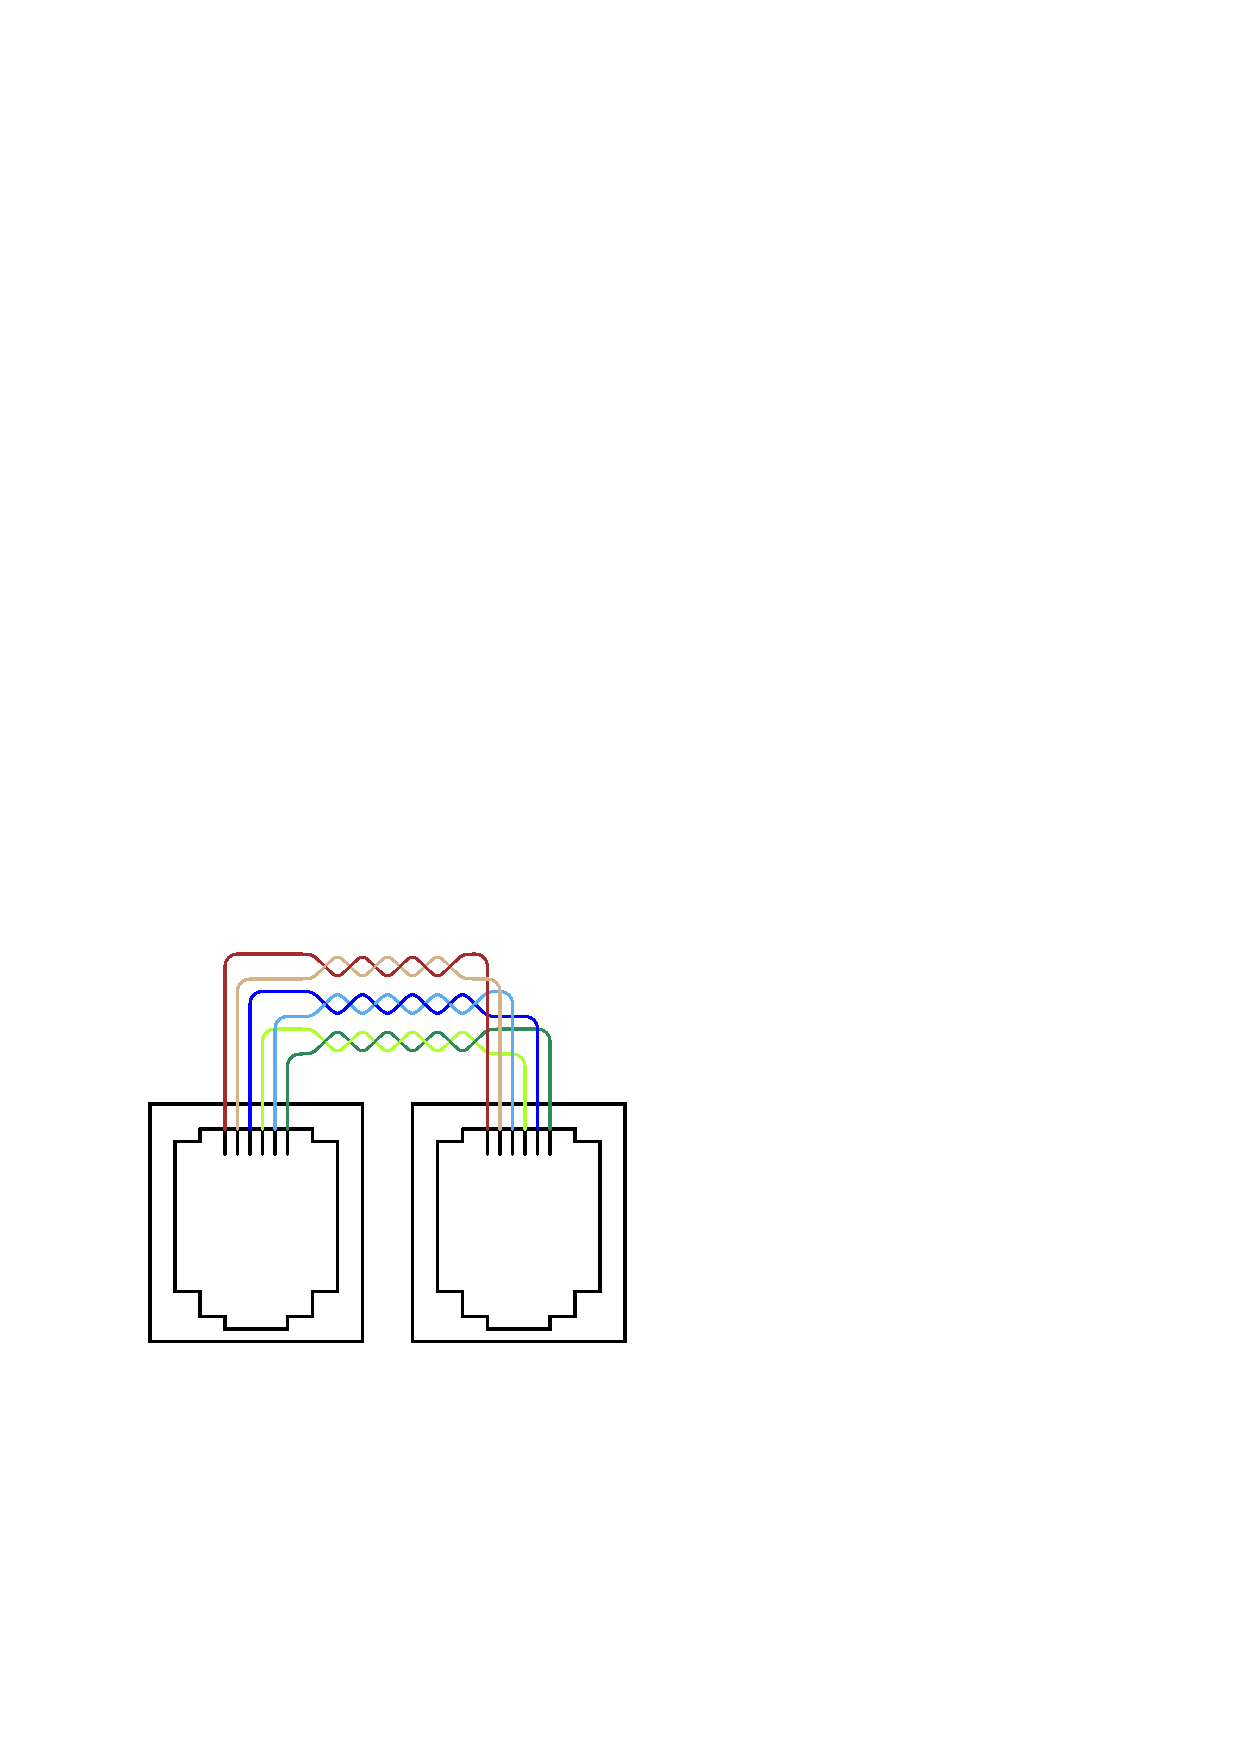
\includegraphics{../media/hbusinterconn.pdf}
\caption{Conexão entre duas portas}
\end{figure}

A recomendação anterior de que o dispositivo possua duas portas deve seguir a regra da conexão cruzada resultando num dispositivo que tem uma porta com o sinal RS485 invertido em relação a outra.

\section{RS485}

O barramento utiliza comunicação RS485 em half-duplex como mencionado. Uma topologia muito comum para drivers é mostrada na figura.

\begin{figure}[H]
\centering
\includegraphics{../media/485drv.pdf}
\caption{Driver RS485}
\end{figure}

É recomendado o uso de um driver integrado deste tipo para a comunicação half-duplex. Há diversas opções de grandes fabricantes de semicondutores. No desenvolvimento foram usados drivers DS75176B.

\section{Alimentação}

A alimentação destinada aos dispositivos conectados ao barramento é de baixa potência devido a limitação imposta pelos condutores. O dispositivo deve ter o consumo mais econômico possível.

No caso de haver necessidade de uma maior potência, o dispositivo deve ser projetado para receber alimentação externa, sendo obrigatório o isolamento do barramento hbus através de soluções como os isoladores de RS-485 da Analog Devices.

Um outro caso é o uso de um repetidor de barramento. Isto é previsto e como é necessária a injeção de corrente, cai na mesma classificação do caso anterior.

Esta especificação não pretende definir limites extremamente rígidos para a tensão de alimentação no barramento, porém por questão de segurança todos os dispositivos devem suportar uma tensão mínima de 24 Volts.
